\begin{figure}[ht!]
\centering
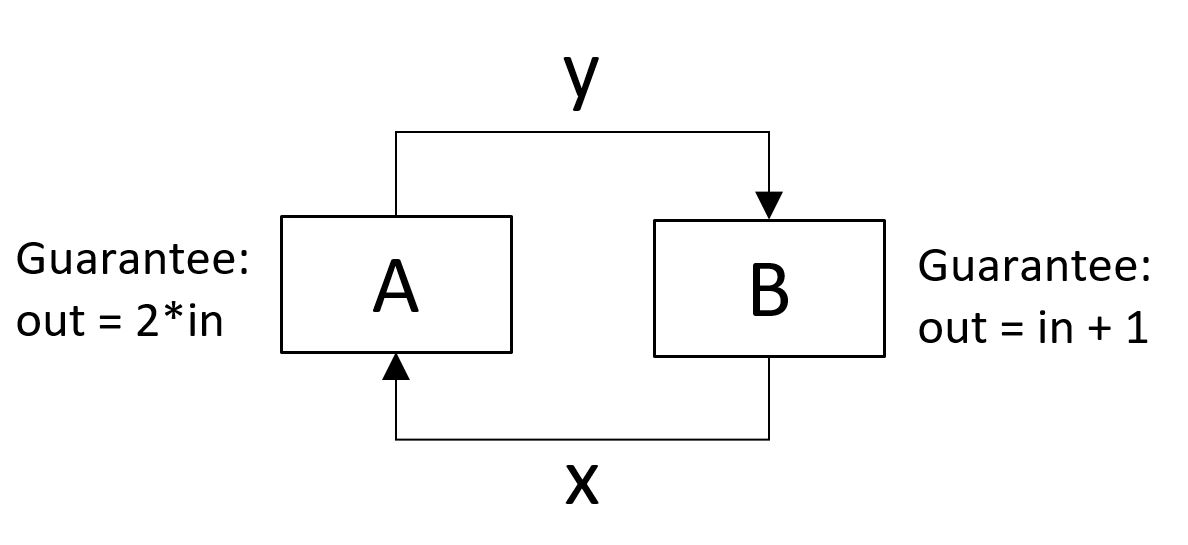
\includegraphics[width=60mm]{simpleFeedback.jpg}
\caption{A Simple Feedback System\label{motivationFig1}}
\end{figure}

We use an example to explain the intuition and illustrate the key sematic difference between the synchronous MoC in original AGREE and the proposed MoC.
Consider an AADL model that consists of two threads $A$ and $B$, as shown in Figure \ref{motivationFig1}. Assume all ports are data ports. The behavior of each thread is indicated by its AGREE contract. Thread $A$ output doubles its input. Thread $B$ output increments its input by one. By the synchronous semantics, the value of signal $x$ and $y$ at instant $n$ is defined by the solution to the two equations $y_n = 2x_n$ and $x_n = y_n+1$, for all $n \in N$. This results in $x = (-1, -1, …)$, $y = (-2, -2, …)$. However, if the two threads execute in a sequential order $(ABAB...)$, and let $x_0, y_0$ denote the initial value of $x$ and $y$, respectively, an intuitive interpretation of the execution semanitcs is $y_1 = 2x_0, x_1 = y_1+1, y_2 = 2x_1...$. If $x_0 = 0$ and  $y_0 = 0$, this results in $x = (0, 1, 3, 7,…)$ and $y = (0, 0, 2, 6, …)$. The example shows that the behavior of a synchronous model is defined by the solution(s) to systems of mathematical equations (or inequalities) at each time instant, while the behavior of the proposed MoC is defined through iterations over time. 

\begin{figure}[ht!]
\centering
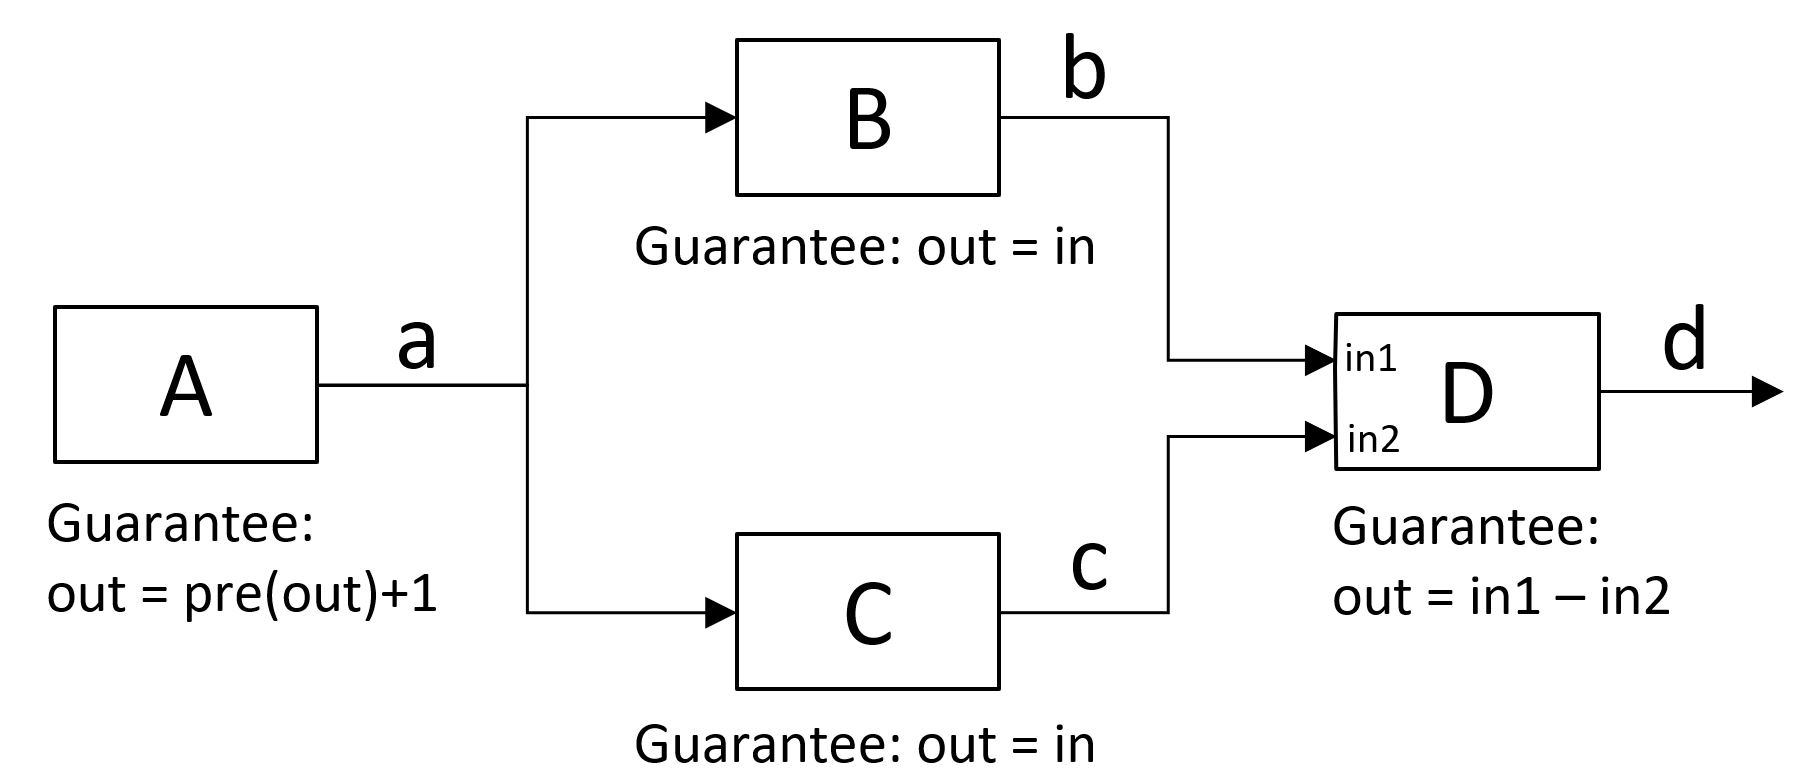
\includegraphics[width=80mm]{downsample.jpg}
\caption{A Simple Downsampling System\label{motivationFig2}}
\end{figure}

Now we use another example to illustrate the motivation of our work.
Consider an AADL model that consists of four threads $A, B, C, D$, as shown in Figure \ref{motivationFig2}. Assume all ports are data ports. Thread $A$ outputs the sequence of all natural numbers. Thread B and thread C simply copy its input to the output. Thread D is a subtractor, where the second (bottom) input value is substracted from the first (top) input value. Given a schedule $(ACABD)^*$, let us say we want to prove that the primary output $d$ is a sequence of ones (ignoring the inital prefix). This can be achieved with the proposed MoC, since thread $B$ only copies even numbers, and thread $C$ only copies odd numbers. However, it cannot be proved directly with the  synchrnous semantics, which results in $d$ as a sequence of zeroes.  To model execution order in a synchronous model, a special construct \emph{delay} is often introduced. However, in the example, thread $B$ and $C$ essetially downsample the data stream from thread $A$. To model this kind of behavior (e.g. downsampling or upsampling), it requires much more complicated modelling mechanism than simple \emph{delays}. 

Note that if the schedule is $(ABCD)^*$, $d$ is a sequence of zeroes (ignoring the intial prefix). This indicates that the execution order could have an impact on the system behvavior. As we will show later, our MoC is not a variant of Kahn Process Network \cite{KPN}, like Lee's Synchronous Dataflow \cite{SDF}, where any execution order results in the same system behavior. Therefore, it makes sense to tie a property proof to a specific schedule.
%Also note that we could add \emph{assumption: input is an even number} to thread $B$. The assumption has no impact on the system behavior under the proposed MoC. However, under the synchronous AGREE MoC the system has no valid behavior. This is because the assumption is violated under the synchronous semantics. This kind of assumptions are not uncommon. It creates a modelling challenge for using synchronous models. 


 
  